El software del nivel supervisor se implementa en Python 3 siguiendo una arquitectura modular que separa responsabilidades en capas funcionales específicas. La Figura \ref{fig:arquitectura_modulos_supervisor} muestra la organización de módulos y sus dependencias.

\textbf{Capa de Hardware}: Gestiona la comunicación con el nivel regulatorio y la adquisición de imágenes. El módulo UARTManager implementa comunicación serial mediante puerto USB a 115200 baudios, utilizando callbacks para procesamiento asíncrono de mensajes recibidos del firmware. El módulo CommandManager proporciona métodos de alto nivel para enviar comandos estructurados al nivel regulatorio.

\textbf{Capa de Control}: Coordina el estado global del robot. El módulo RobotController mantiene el seguimiento de posición global mediante acumulación de desplazamientos reportados por el firmware, detecta y maneja eventos mediante callbacks, y gestiona la persistencia de estado en archivos JSON. El módulo CameraManager centraliza el acceso a la cámara USB evitando conflictos de acceso concurrente.

\textbf{Capa de Robot}: Implementa el control del brazo robótico. El módulo ArmController define cuatro posiciones operacionales discretas con ángulos específicos de servomotores y genera trayectorias mediante interpolación lineal.

\textbf{Capa de Procesos}: Define las secuencias de alto nivel del robot. El módulo workflow\_orchestrator implementa los cuatro procesos principales del sistema: homing, calibración del workspace, mapeo del entorno, y cosecha interactiva.

\begin{figure}[H]
    \centering
    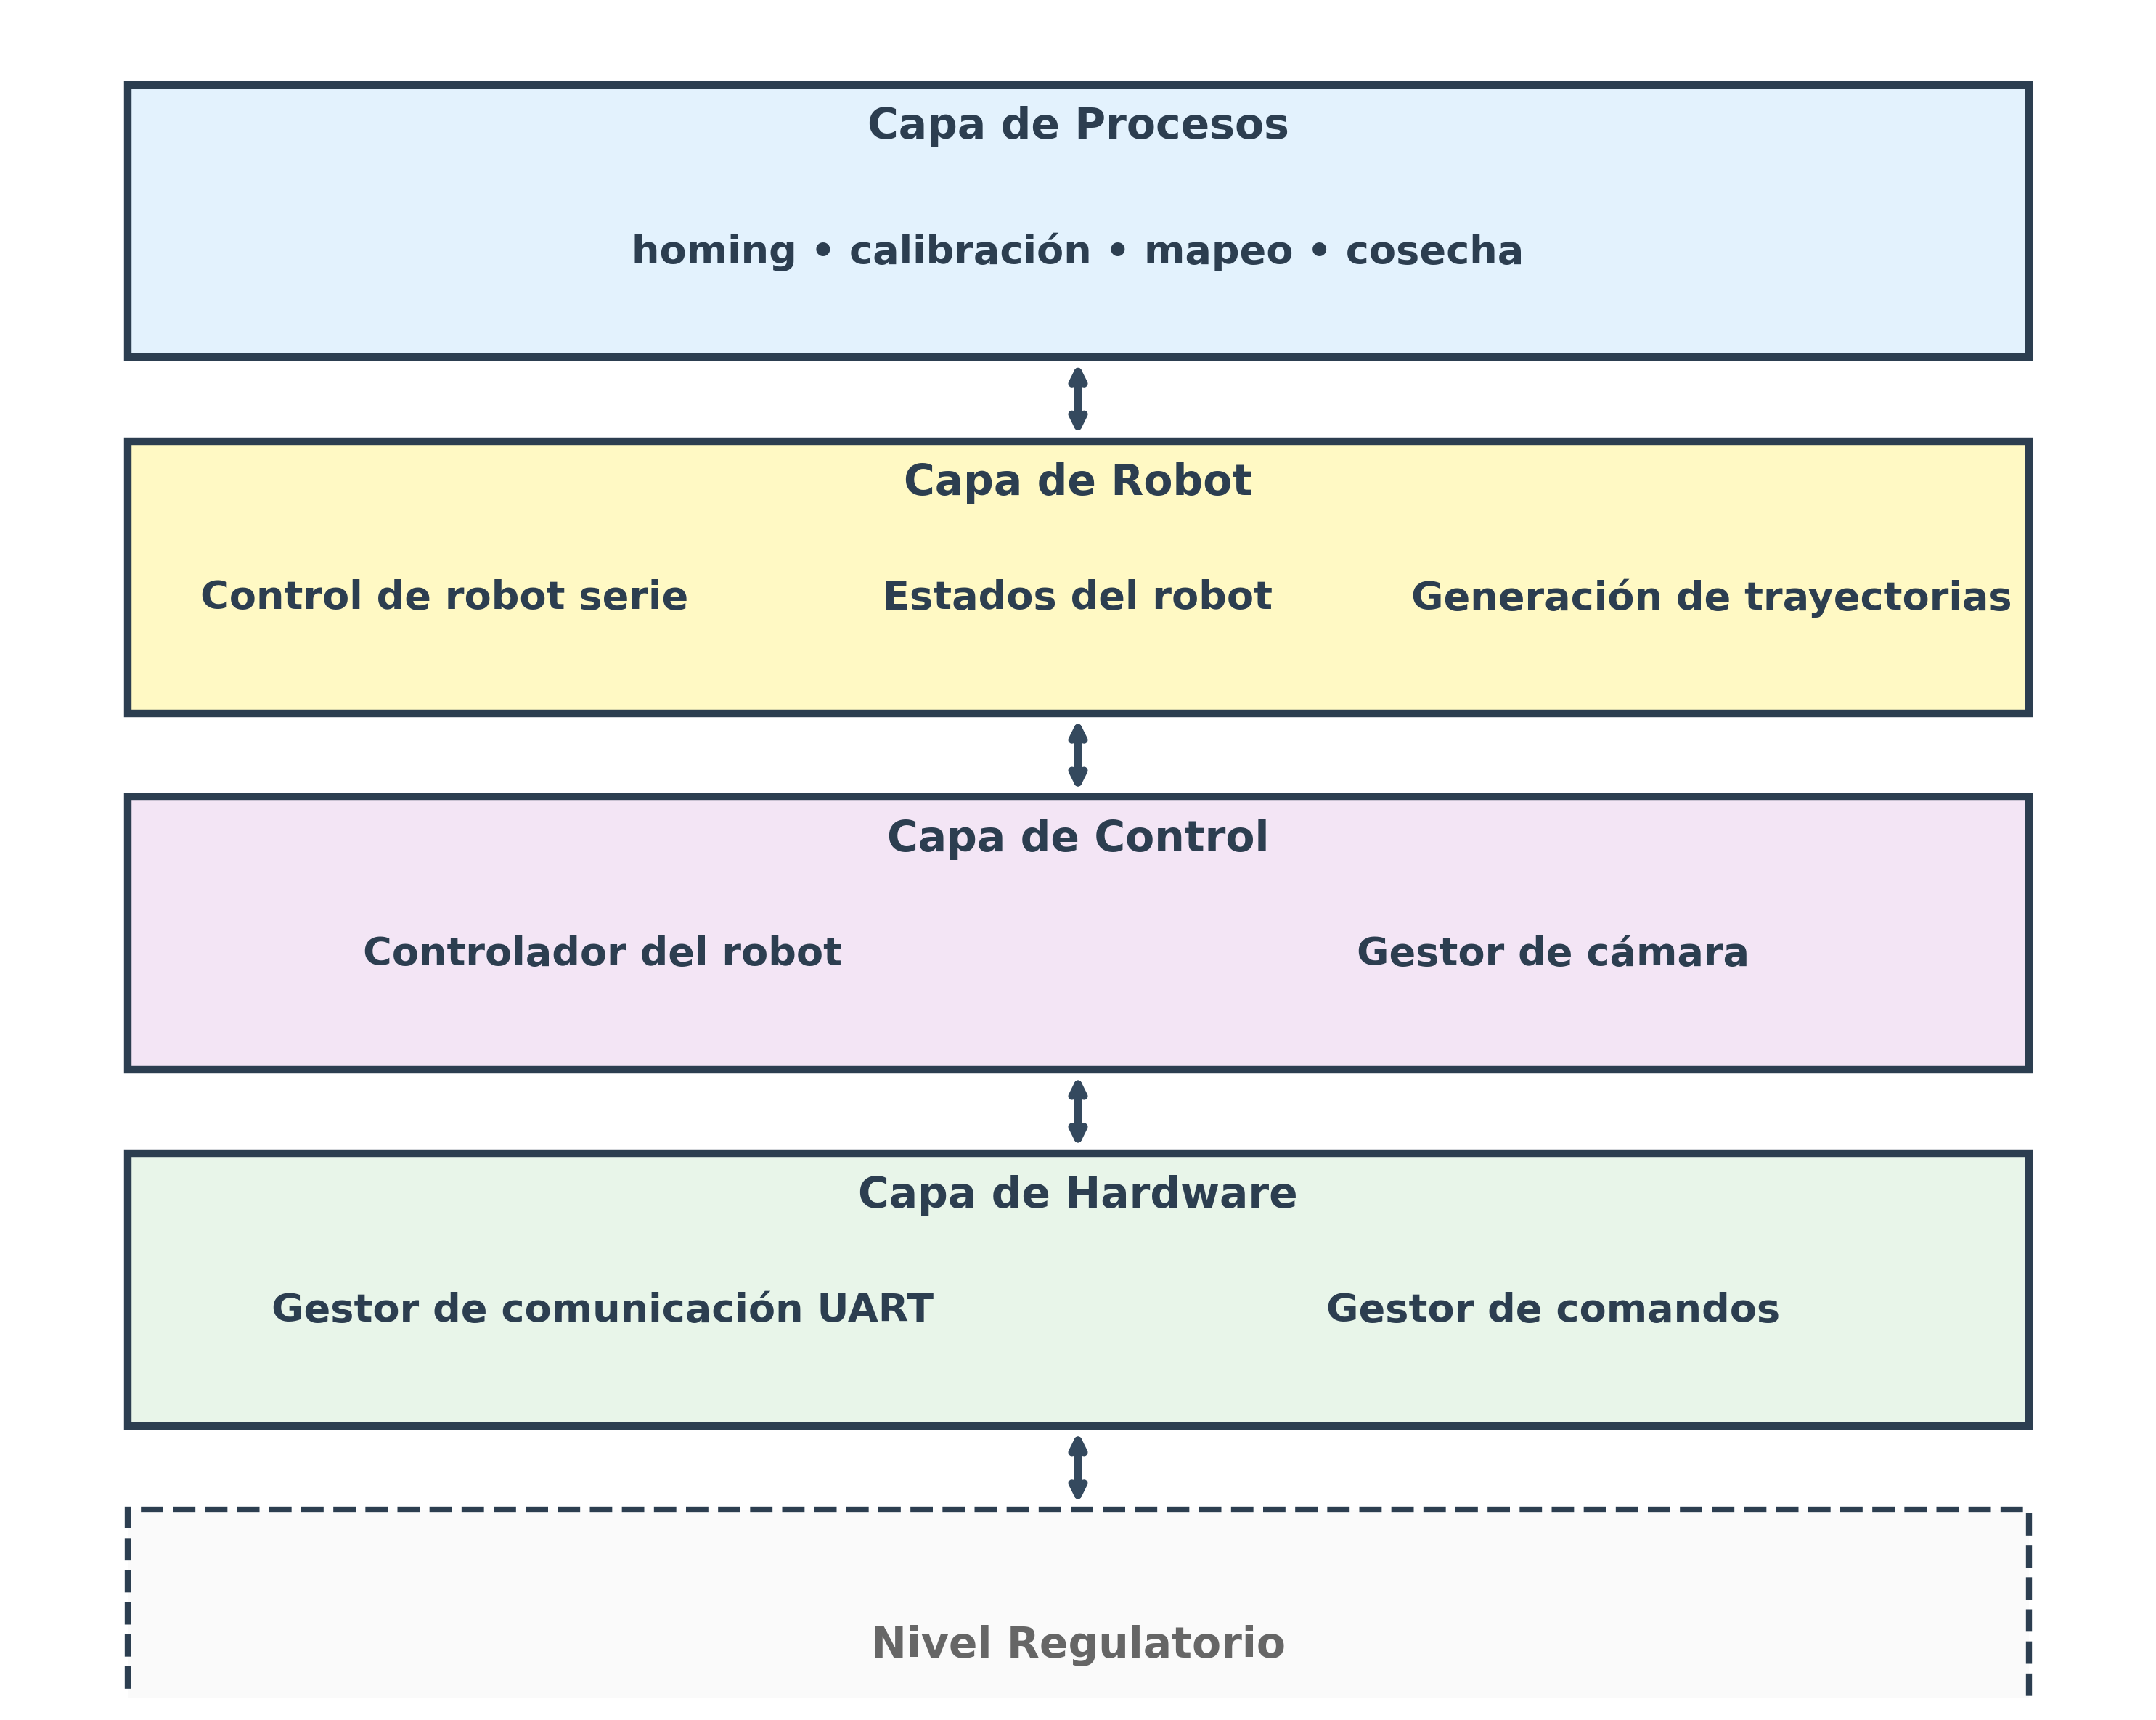
\includegraphics[width=0.8\textwidth]{imagenes/arquitectura_modulos_supervisor.png}
    \caption{\textit{Arquitectura modular del software supervisor mostrando capas y flujo de información}}
    \label{fig:arquitectura_modulos_supervisor}
\end{figure}